\section{Literature Review}
\subsection{Introduction}
Research on abstractive text summarisation (Sec. \ref{textsum}) for article headlines has been primarily undertaken by industry in recent years, with progress being made by Facebook~\cite{Rush2015,Chopra2016}, Google~\cite{Liu2016}, and IBM~\cite{Nallapati2016a}. As stated in Sec.~\ref{intro}, these approaches all implement attentional seq2seq (Sec.~\ref{seq2seq}) models, which generate a sequence of words from a different sequence of words. An important open question in seq2seq design, however, revolves around a concept called teacher forcing. To understand the scope and implementation of this work, a review of text summarization, deep neural networks, recurrent neural networks, seq2seq attentional models and teacher forcing techniques is provided.

\subsection{Text Summarization}\label{textsum}
Computer Scientists have been working on automated text summarization techniques since 1958~\cite{Luhn1958}. Within the subfield, there are two broad categories: extractive and abstractive. Extractive summarization attempts to evaluate the most important words, phrases, and/or sentences within an article and reconstruct a short summary using computational linguistics to place words in the correct order for the summarization. This, however, often leads to very unnatural sounding headlines and relies entirely on words present within the article~\cite{Radev2002}. There are simply too many nuances in languages to account for every possible syntactic structure.

Abstractive summarization, by contrast, attempts to view patterns within the article relative to other articles it has seen. It then attempts to generate a summary based upon these patterns and does not rely upon any of the words in the article for constructing its summary.  Abstractive summarization is much more akin to human-esque comprehension, reads more naturally and has eluded researchers for decades. In his 2002 descriptive paper, Radev goes so far as to say ``true abstractive summarization remains a researcher's dream''~\cite{Radev2002}. With the renaissance that deep learning has witnessed within the past few years, however, this is beginning to look like a possibility. As such, this project will focus on abstractive summarization contribution.

\subsection{Deep Neural Networks}\label{dnn}
DNNs are one of the most widely used machine learning tools today. Some of their most notable achievements have been the identification of objects in images~\cite{LeCun1989}, language comprehension and translation\cite{Mikolov2010,Mikolov2011}, and even mastering some of the world's most difficult board games~\cite{Silver2016}. Their development was inspired by the synaptic connections of biological neurons, which have continued to serve as inspiration~\cite{Schmidhuber2015}. Neurons receive information from environmental input, such as sight, and proceed to pass and receive electrical signals to and from other neurons via axons to process the input. Eventually, after thousands of passes through different neurons (of which there are approximately 100 billion in the human brain)~\cite{Goodfellow2016}, an understanding of the input is arrived at.

\begin{SCfigure}[1][h]
  \caption[Example of a biological neuron]{Example of a biological neuron. Neurons carry information along their axons to other neurons using synapses. These neurons then transfer this electrical signal to another neuron and so forth. From~\cite{NationalInstituteofAging2011}.}
  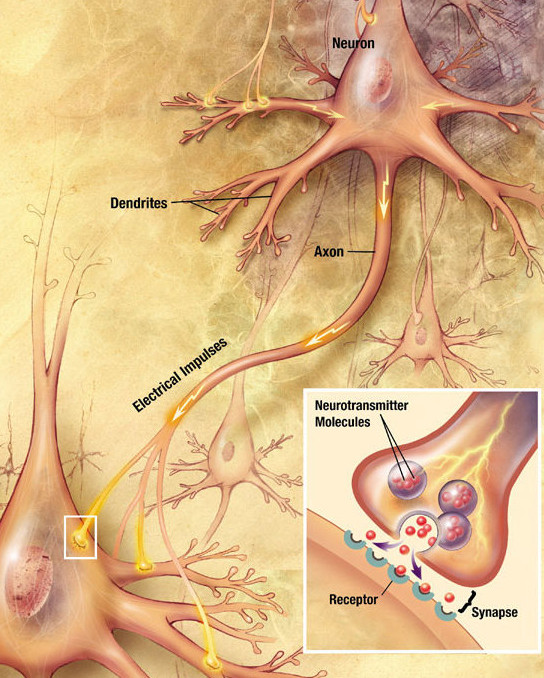
\includegraphics[width=0.3\textwidth]{synapse}
  \label{fig:synapse}
\end{SCfigure}

DNNs can be applied to all three broad machine learning categories: supervised (SL), unsupervised (UL) and reinforcement (RL). The most common is SL, in which the expected output of the model is known and can be used to compare against and adjust the machine learning algorithm's hypothesis. Furthermore, in practice, DNNs have two broad categories: recurrent and convolutional. The former ensures a maintenance of state for successive timesteps, while the latter, used primarily in image recognition and generation, is adept at discovering complex patterns.  As seq2seq is a supervised recurrent method, this discussion will be focused on the respective machine learning techniques.

As mentioned previously, DNNs draw inspiration from biological neurons, containing an input layer, hidden layers, and an output layer with numerous nodes in each. Every node, aside from those in the output, relays information to every other node in the proceeding network layer. These nodes simulate the neurons, with connections between them representing axons and synapses.

\begin{figure}[h]
  \centering
  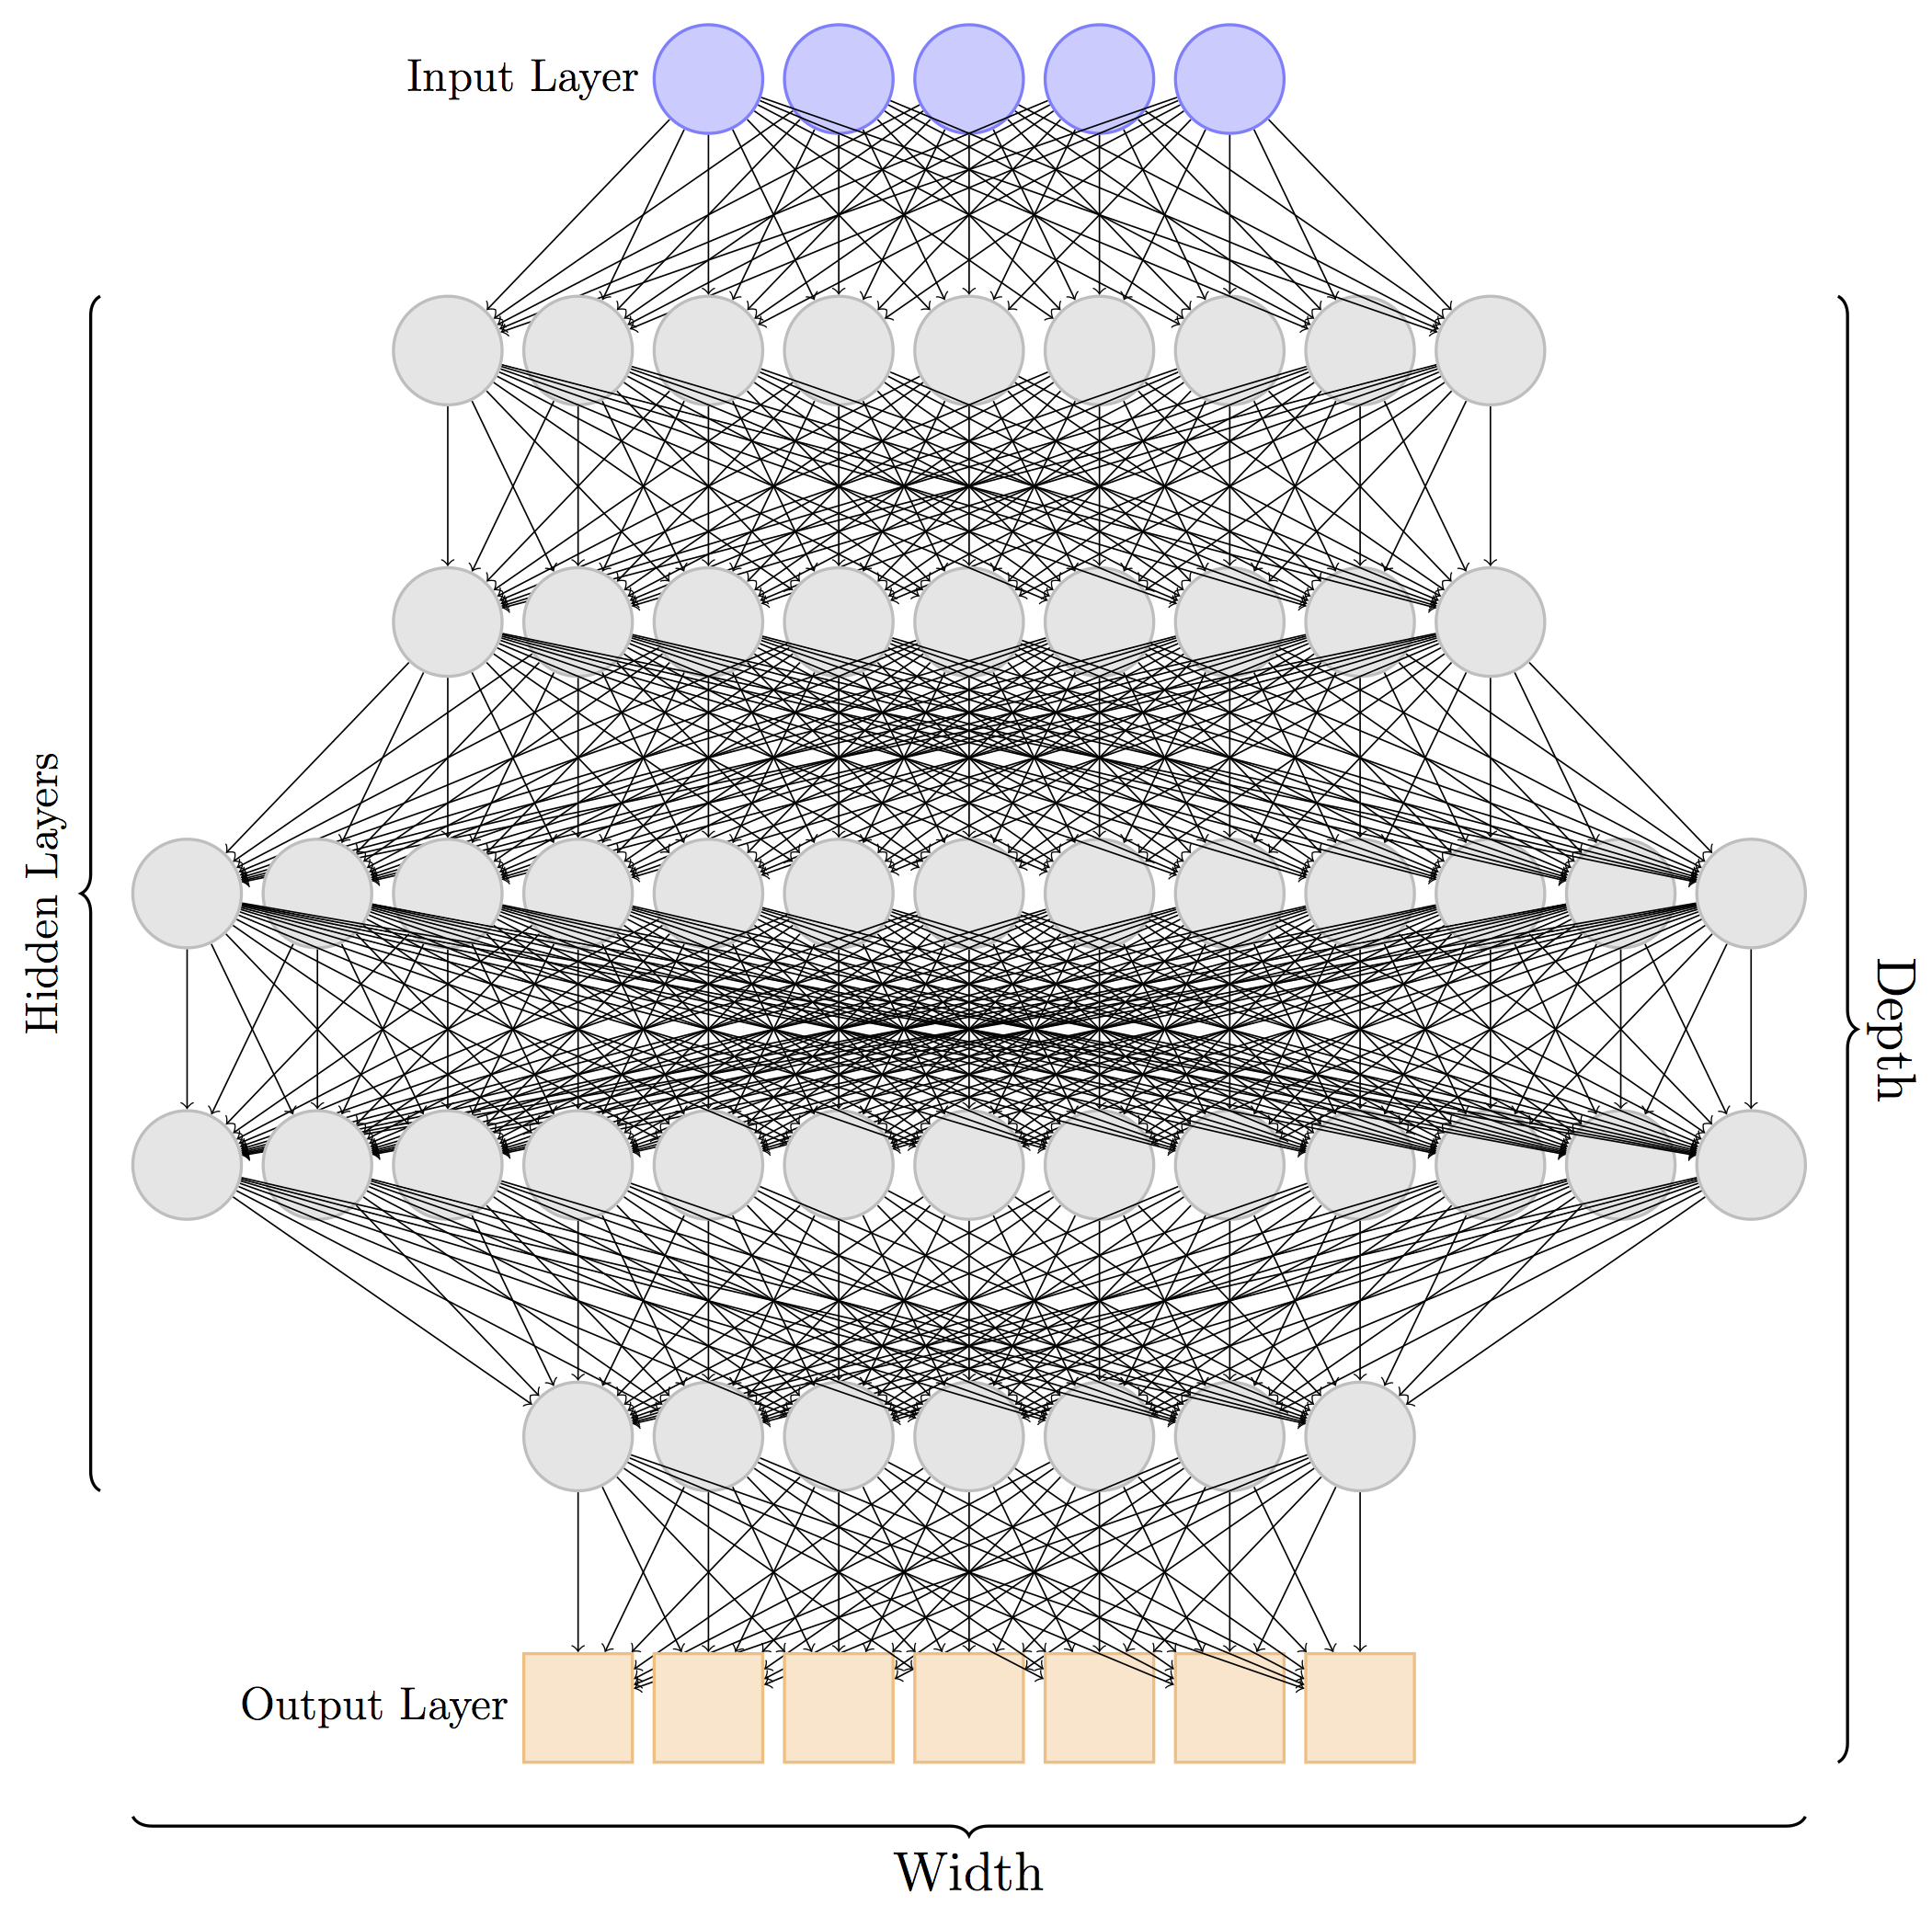
\includegraphics[width = 0.75\textwidth]{nngraphics}
  \caption[Six layer deep neural network]{A six layer deep neural network. NB:\@ANN Architectural naming convention does not include the input layer~\cite{Stanford2016}}
  \label{fig:NNDiagram}
\end{figure}

First, there is an input layer. This is where the pixel values of an image, or the embeddings (See Sec.~\ref{emb})  of a word in the source sentence of a translation would be fed. There are a series of hidden layers of varying, arbitrary width. A neural network is “deep” if it has multiple layers (though how many designates an architecture as deep is up for debate). Finally there is an output layer, which could be anywhere from a single node representing a prediction for the next word in a sentence, to a series of nodes detailing what percentage it believes this image is a shoe, a football or a saxophone. So the number of nodes in the input layer and output layer are predetermined based upon the problem you are trying to solve, but the intermediate architecture is up to the neural network designer.

\subsubsection{Forward Propogation}
An important insight into understanding DNNs is realizing that they are simply a set of matrix multiplications followed by transformation functions. To begin, the input layer passes its values, multiplied by a set of weights, to every node in the next layer. These weights can intuitively be thought of as a level of importance (this is not accurate, but can help in comprehension). Each node now contains a new value. This value is then transformed, generally using a method called ReLU, which is short for Rectified Linear Unit. This simply means the greater of 0 and the value, or $max(0,x)$~\cite{Nair2010}.

At this point, the input has been transformed into the first hidden layer. This process is repeated by each successive layer until you get to the output layer. The activation function for the output layer is going to be different and tailored to the specific problem. In the case of seq2seq problems, a sigmoid function, $f(x) = \frac{1}{1+e^x}$, will output a percentage value for what the neural network believes is most likely to be the next word in the sequence. The maximum value will then be selected. So by the time we have reached the output layer, a long string of various matrix multiplications and ReLU transformations has occured. The output layer is simply a function of many other functions of functions. Arriving at the output completes the forward propogation of a single training example.

The reason for the high degree of effectiveness of DNNs is that they can model every function at extremely high dimensionalities~\cite{Nielsen2017}. This was the crucial insight into being able to leverage neural networks for such a wide range of problems. Simply by multiplying by a set of weights and transforming with an activation function several times, extremely complex functions can be modeled to a high degree of accuracy.

\subsubsection{Cost Calculation}
The magic of neural networks is in the weights that each successive layer is multiplied by before being transformed by the activation function. The correct values for these weights are what DNNs are trying to learn.  When DNN models are first created, these weights are initialized randomly, so the model will have no predictive capability whatsoever at this point. The prediction will be compared to the actual value, or the next word in the sentence, as is the case with seq2seq. The cost function is generally cross entropy loss, which has the benefits of being positive and trending towards zero as the loss decreases~\cite{Nielsen2017}. The specifics of the cost function are not important, but it is critical to understand that when a prediction is wrong, the value of the cost function is greater than zero. By adjusting the weights in each layer, this cost function can be minimized.

\subsubsection{Backpropogation}
To ensure the weights are changed in the correct direction, backpropogation is used. After the cost function has been calculated, we can take the derivatives of the function described by the current neural network to find the slope of the cost function for all current weights. By using the chain rule to propogate backwards through the entire function, we can find the slope of the cost. If there is a slope to the cost function, this means the cost can be less than it currently is and a small step in the right direction towards minimizing this cost can be achieved.

\subsubsection{Gradient Descent}\label{grad}
Now that the derivatives have been calculated, a small step towards the minima of the cost function is taken by modifying the weights in the correct direction as deteremined by backpropogation. The size of these steps is determined by a learning rate, which generally must be lowered as the model becomes more and more accurate. There are various methods for calculating this, and intricacies such as momentum to accelerate the learning process, but these are not important for understanding the core concepts. If learning is done one training example at a time, it is called stochastic gradient descent. Eventually, after several epochs (Forward Propagation, Cost Calculation, Backpropogation and Gradient Descent on the entire training dataset), the DNN will have learned the optimal set of weights to minimize the cost function and make accurate predictions or classifications.

\subsubsection{DNN Conclusion}
Stated simply, DNNs are a series of layers that contain weight matrices that each modify the previous layer before undergoing a transformation. Eventually this produces an output that at first is very wrong, but by taking the derivative of the cost function applied to every layer and minimizing the loss accordingly, DNNs can be trained to be highly accurate machine learning tools. The example presented above is a simple, fully-dense DNN with only one input layer and no sense of state. The previous prediction has no bearing on the next prediction. For understanding the sequence of words in an article, however, a sense of state is important---a problem solved by RNNs~\cite{Elman1990}.

\subsection{Recurrent Neural Network}\label{rnn}
RNNs are so-called because they feed the state of the previous timestep calculation into the next state. This can best be visualized in Figure~\ref{fig:rnn}. Here, you can see a sequence of inputs, $X_{0...t}$, that are fed into a hidden state that derives information from the hidden states of previous timesteps.

\begin{figure}[h]
  \centering
  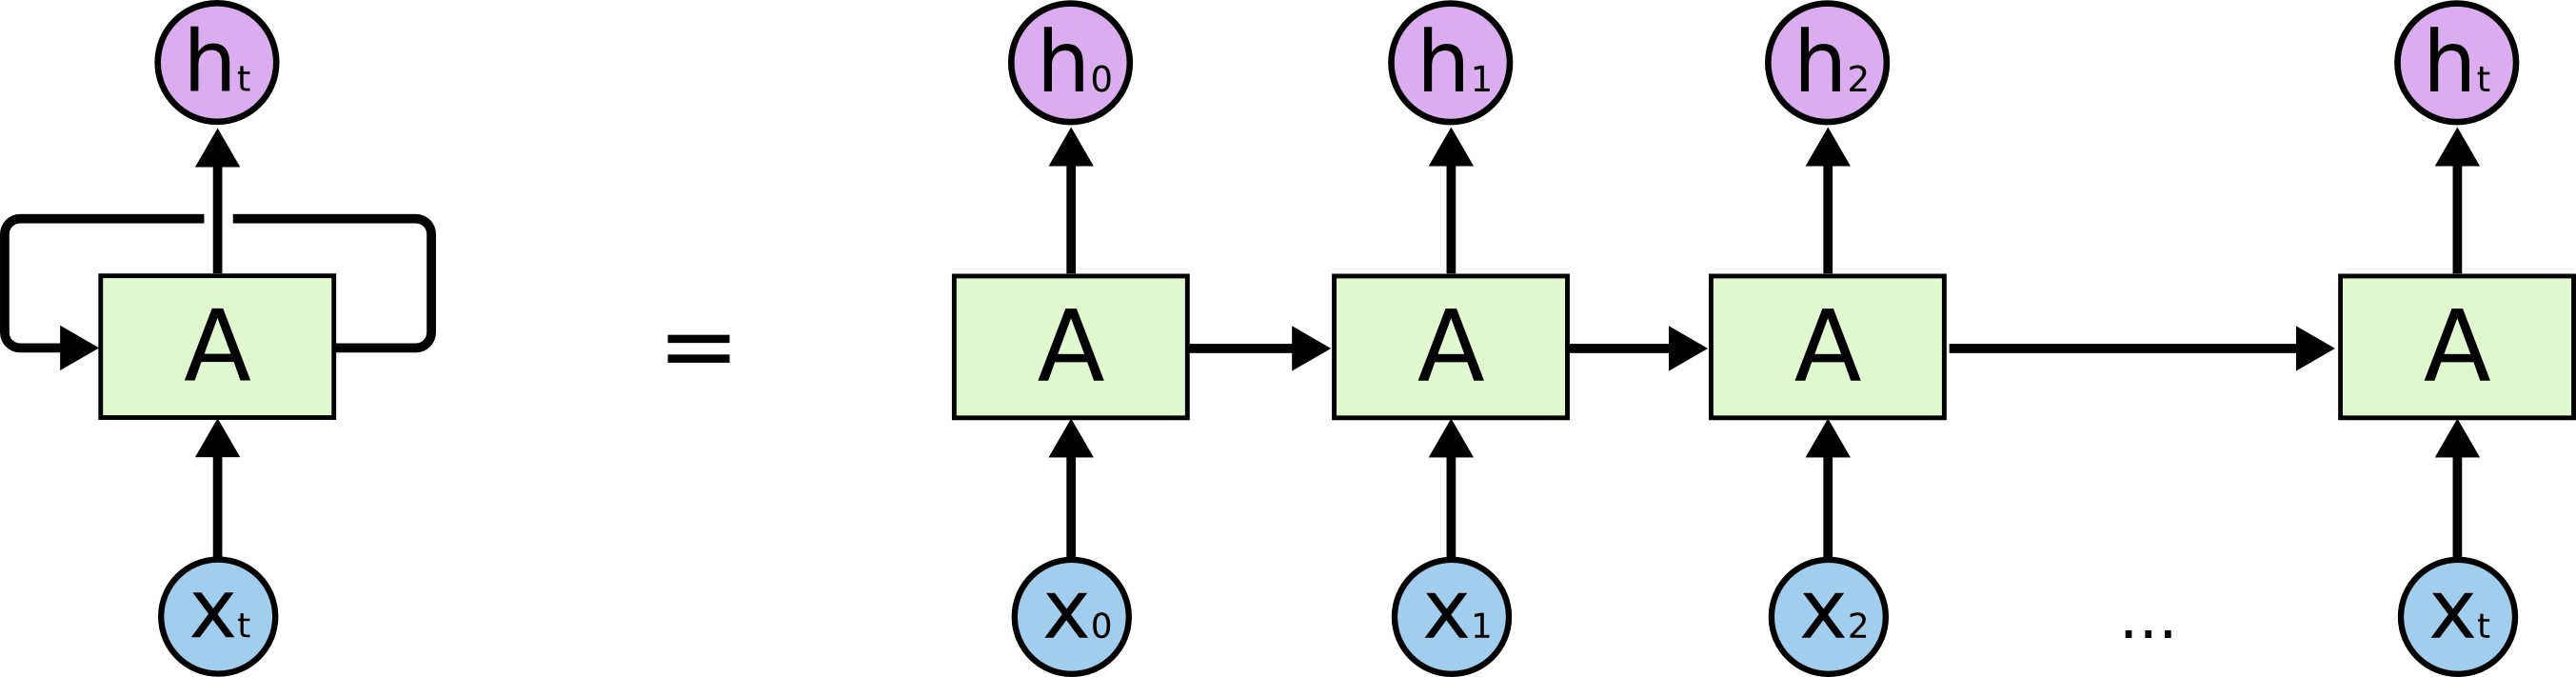
\includegraphics[width=0.7\textwidth]{RNN-unrolled.png}
  \caption[Single layer RNN]{A depiction of a simple, single layer RNN. On the left is the traditional representation which can be unrolled as displayed on the right side of the image. From~\cite{Olah2015} with permission.}
  \label{fig:rnn}
\end{figure}

This combination of new input and old state being input into the new hidden state allows for the model to develop a sense of context from the previous timesteps. To understand this concept of timesteps, imagine the following input sentence (the first sentence is often all that is used in modern headline length article summarization~\cite{Liu2016,Rush2015,Chopra2016,Nallapati2016a}): ``New research from XYZ suggests that quick brown foxes have been jumping over lazy dogs at an alarming rate.'' Each individual word would be the input at it's respective timestep, so $X_0$ = 'New', $X_1$ = research, and so forth. In NLP, there are two types of RNNs: character and word. In the case of a character-RNN, this sequence would have 107 timesteps, one for each subsequent character, including spaces and punctuation. A word-RNN would have 20 timesteps. As in DNNs, the hidden states that these inputs are fed into have a set number of nodes that contain an associated weight. Because they continually recieve context from previous timesteps, RNNs can learn spelling, punctuation, and grammatic and syntactic structure without ever being explicitly trained~\cite{Karpathy2015}.

The original conception of an RNN contained only a simple transformation, as displayed in Figure~\ref{fig:simprnn}.

\begin{figure}[h]
  \centering
  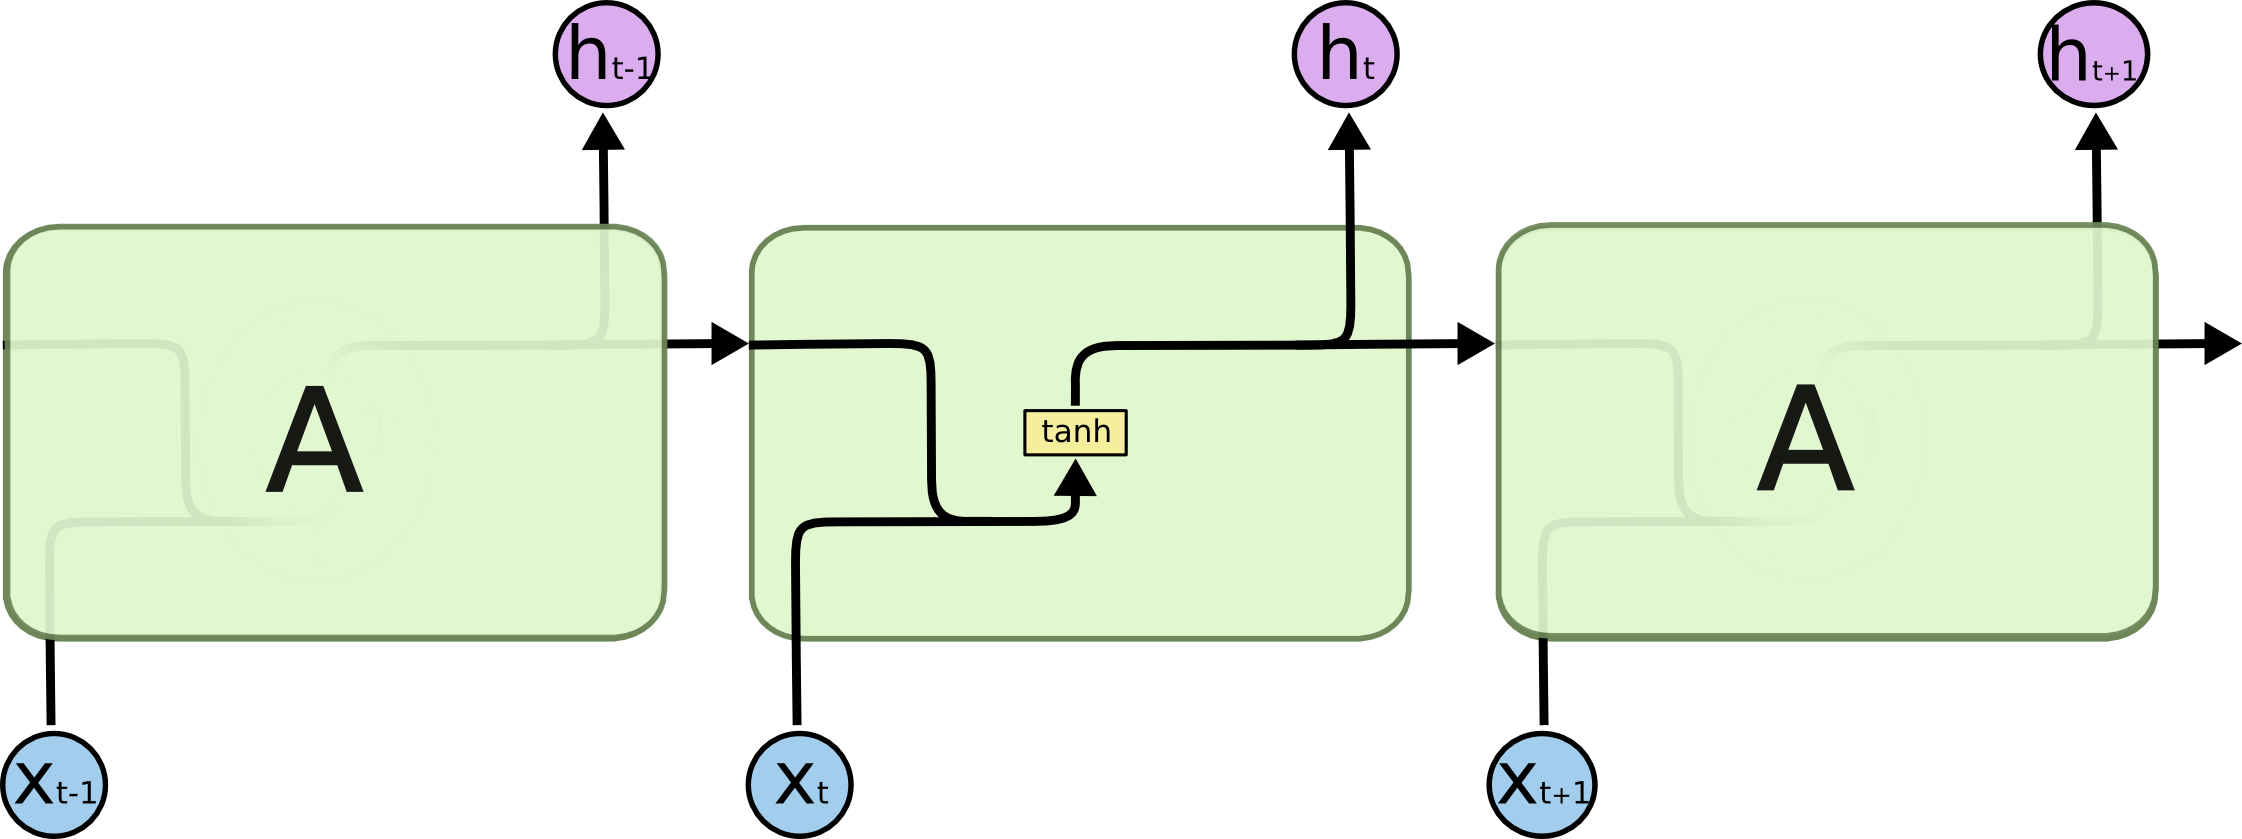
\includegraphics[width=0.65\textwidth]{SimpleRNN}
  \caption[RNN Mechanics]{The inner-workings of the hidden state for traditional RNNs. From~\cite{Olah2015} with permission.}
  \label{fig:simprnn}
\end{figure}

In theory, this simple structure should have worked, but in practice, problems such as exploding gradients prevented them from converging (minimizing the loss function to a stable, low overall cost) during training \cite{Hochreiter1991,Bengio1994}. As a result, much research was undertaken to solve this issue, leading to the development of Long Short-Term Memory (LSTM) networks~\cite{Hochreiter1997}, which have since become the defacto standard~\cite{Karpathy2015}.

\subsubsection{Long Short-Term Memory}\label{lstm}
LSTMs are a significantly more complex type of RNN, as seen in Figure~\ref{fig:lstm}.

\begin{figure}[h]
  \centering
  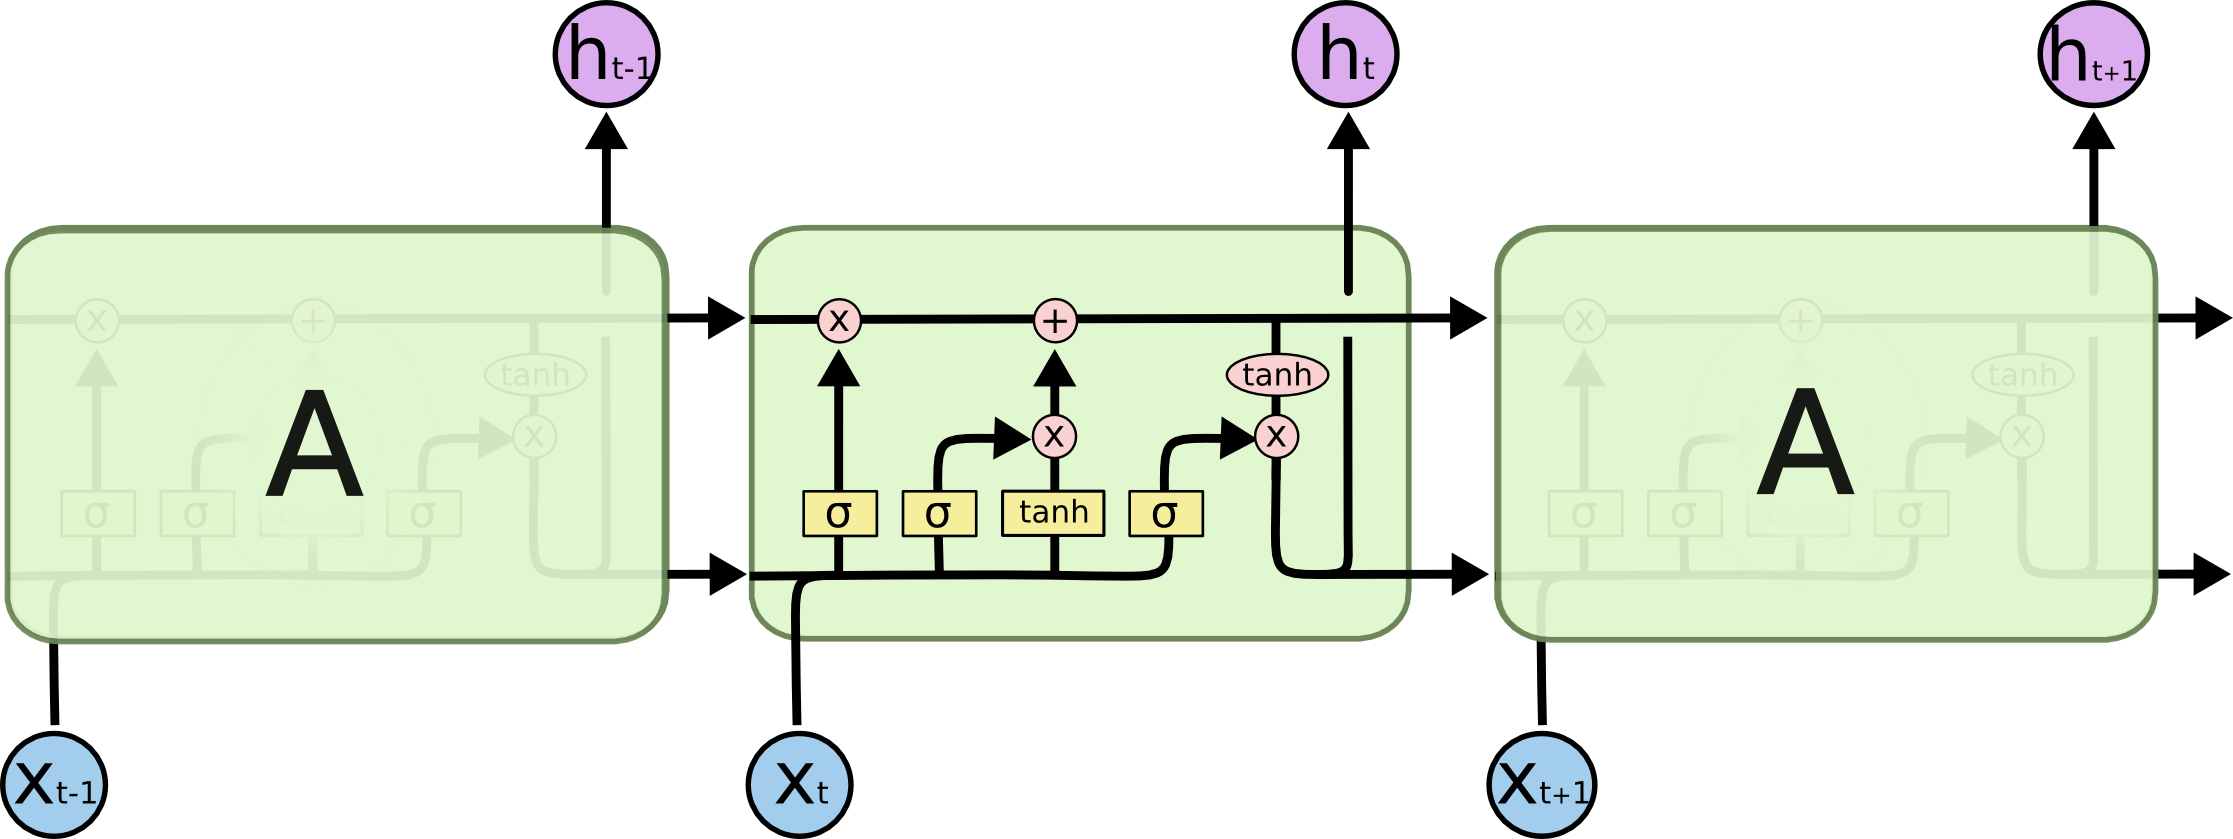
\includegraphics[width=0.65\textwidth]{lstm}
  \caption[Original LSTM]{The original LSTM as described in~\cite{Hochreiter1991}. From~\cite{Olah2015} with permission.}
  \label{fig:lstm}
\end{figure}

The details are not significantly important, but the main takeaway is that LSTMs essentially contain miniature neural nets that dictate how much information should flow from certain outputs to the next, called sigma ($\sigma$) gates. These $\sigma$ gates output a value between one and zero to determine the amount of information released to the main hidden state channel, represented by the horizontal bar running across the top of Figure~\ref{fig:lstm}~\cite{Hochreiter1991,Olah2015}. In this way, a more complex sense of state can be achieved.

\subsubsection{Gated Recurrent Unit}\label{gru}
The LSTM architecture, developed in 1997, was the only RNN architecture used in practice until 2014~\cite{Karpathy2015} when the Gated Recurrent Unit was developed by~\cite{Cho2014}. It simplified the LSTM by combining certain functions and getting rid of others.

\begin{figure}[h]
  \centering
  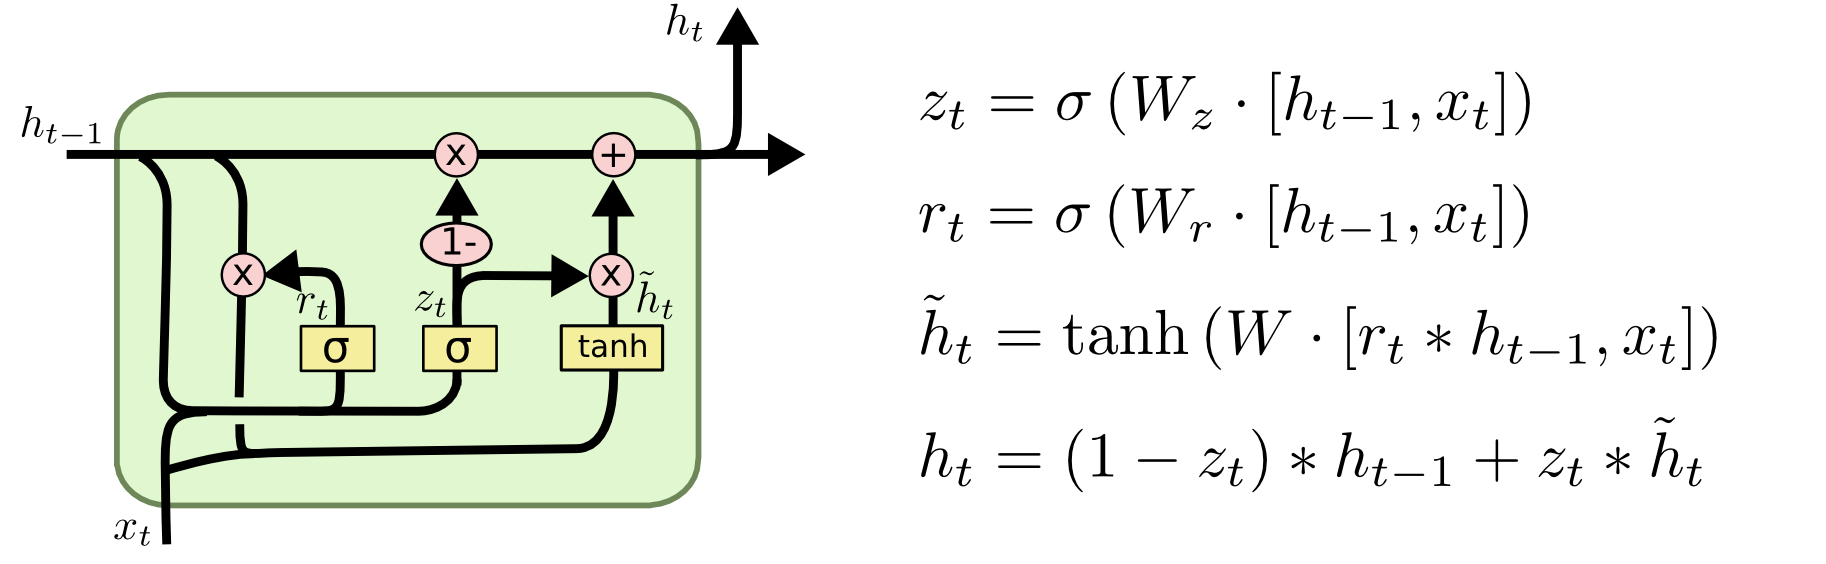
\includegraphics[width=0.65\textwidth]{gru}
  \caption[GRU]{The GRU as described in~\cite{Cho2014}. From~\cite{Olah2015} with permission.}
  \label{fig:gru}
\end{figure}

Again, the specifics are not important, but it is important to know that these have become a popular option for RNN architectures. As regards effectiveness, both LSTMs and GRUs seem comparable on average and appear very task dependent~\cite{Jozefowicz2015,Greff2016}. However, because GRUs are slightly simpler and consequently take less time to train, these are more often used than LSTMs.

\subsubsection{Bidirectional RNN}
RNNs as pictured in Figure~\ref{fig:simprnn} only send state in one direction. So, the first word has no context for later words in the sentence. This is ultimately unhelpful, as oftentimes the words picked at the beginning of a sentence are dependent upon the rest of the sentence structure. To address this, bidirectional RNNs were developed~\cite{Schuster1997} as displayed in Figure~\ref{fig:bidir}.

\begin{figure}[h]
  \centering
  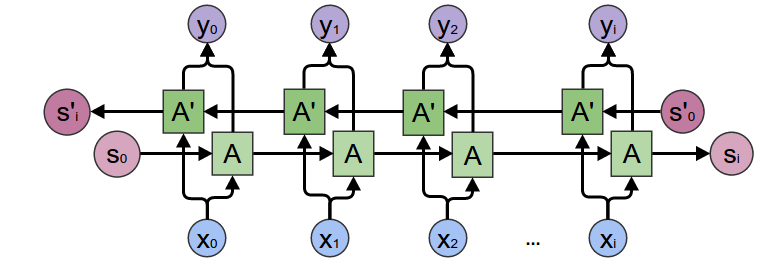
\includegraphics[width=0.5\textwidth]{RNN-bidirectional}
  \caption[Bidirectional RNN]{A bidirectional RNN. From~\cite{Olah2015} with permission.}
  \label{fig:bidir}
\end{figure}

A bidirectional RNN is just a standard RNN merged with another RNN running through the sequence backwards to ensure that each timestep contains state information about each element both preceeding and proceeding it. These have become the defacto RNN structures used in seq2seq.

\subsubsection{Word Embeddings}\label{emb}
As a final detail to RNNs, it should be noted that an index to a word is not typically fed into the RNN. Instead, an embedding~\cite{Mikolov2000} is created for each word. An embedding is a vector of arbitrary dimensionality that is used to describe characteristics of the word. The values in these vectors will ultimately allow the model to understand whether a word is a noun or an adjective, syntactic structure between words, and any other nuance of language that it can determine from seeing words in differing contexts millions of times~\cite{Bengio2003}. This allows for a word to have dimensionality, which can be thought of as the characteristics of the word. So instead of feeding a word index to an RNN, a vector of learned weights for each individual word is used as the input.

Understandably, the same word across domains often has the same contextual meaning, so it is not necessary to train all words from scratch. Resources like Stanford NLP's GloVe Embeddings~\cite{Pennington2014} and Google Brain's word2vec~\cite{Mikolov2013} have trained word embeddings on dozens of thousands of words across extremely large databases. This allows DNN Engineers to save valuable time training their networks if the Embeddings have already been learnt. It will likely require some tuning after the model has converged, but this will be minimal.

\subsubsection{RNN Conclusion}
RNNs are used to pass a sense of state from timestep to timestep. These, like any DNN architecture, can be stacked on top of one another for increasingly complex pattern recognition and generation, but due to the complexity of their state-maintenance, they take a very long time to train. There are likely some critical pieces of the puzzle we have yet to solve as regards RNNs, but this is the current state of top-performing NLP RNN architectures. A few more levels of complexity are necessary for seq2seq, which will be dissected presently.

\subsection{Sequence-to-Sequence}\label{seq2seq}
Seq2seq~\cite{Sutskever2014} is the primary method used in NLP for turning one sequence of characters into another sequence. Developed in 2014, it is used heavily in Neural Machine Translation~\cite{Bahdanau2014,Wu2016}, speech recognition~\cite{Bahdanau2016}, video captioning~\cite{Venugopalan2016}, and of course, abstractive text summarization~\cite{Rush2015,Chopra2016,Lopyrev2015,Liu2016,Nallapati2016a}. They consist of two primary pieces---the encoder and decoder, as shown in Figure~\ref{fig:seq2seq}.

\begin{figure}[h]
  \centering
  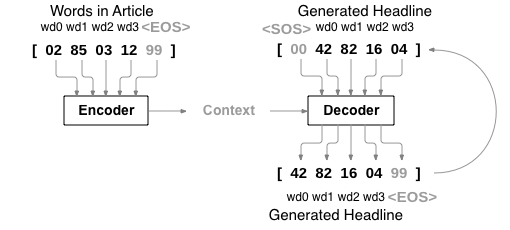
\includegraphics[width=0.5\textwidth]{seq2seq}
  \caption[Basic seq2seq model]{A basic seq2seq model for translating French into English. From~\cite{Robertson2017} with permission.}
  \label{fig:seq2seq}
\end{figure}

The first work on headline-length summarization by~\cite{Rush2015} used a convolutional neural network (CNN) for the encoder and a context-sensitive feedforward network for the decoder. This was expanded upon by~\cite{Chopra2016}, which maintained the use of the CNN for the encoder, but switched to an RNN for the decoder. Today's highest performing architectures, however, use RNNs for both the encoder and decoder~\cite{Hu2015,Nallapati2016a,Liu2016}.

\subsubsection{Encoder}
The encoder takes the input sentence and converts it into a vector representation, denoted by \textit{Context} in Figure~\ref{fig:seq2seq}. By training on thousands, if not millions, of examples the encoder will have learnt how to convert a sentence into a meaningful vector representation, symbolizing the ``essence'' of the input sentence. Obviously, the larger this vector is, the more complex and precise the representation is for any given input.

\begin{figure}[h]
  \centering
  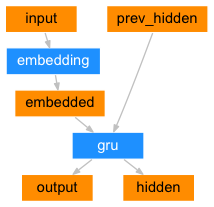
\includegraphics[width=0.3\textwidth]{encoder}
  \caption[Seq2seq encoder diagram]{Diagram of an RNN encoder network. From~\cite{Robertson2017} with permission.}
  \label{fig:encoder}
\end{figure}

While the simple RNN in Figure~\ref{fig:simprnn} produced an output at every timestep, this RNN simply continues to feed its previous state into the next timestep to create the context vector.

\subsubsection{Decoder}
The context vector created by the encoder is then fed as the input to a decoder RNN, the functions of which can be visualized in Figure~\ref{fig:decoder}.

\begin{figure}[h]
  \centering
  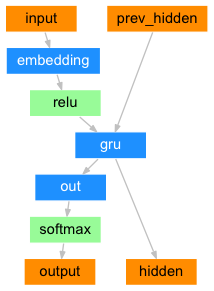
\includegraphics[width=0.3\textwidth]{decoder}
  \caption[Seq2seq decoder diagram]{Diagram of an RNN decoder network. From~\cite{Robertson2017} with permission.}
  \label{fig:decoder}
\end{figure}

At the first timestep of the decoder, a start-of-sentence token, $<SOS>$,will be fed as an additional input. This signals the decoder to predict the first word of the output. In a fully trained seq2seq model, this first word prediction would then be fed into the second timestep, along with the context vector to generate the next word in the sequence. It will continue to do this until the model decides to generate an end-of-sentence token, or $<EOS>$. This then produces the resultant sequence in the seq2seq model.

However, before it has been trained, none of the weights will contain meaningful information for proper sequence generation. This means that during training, you must feed the correct input to the decoder for each timestep and allow it to calculate its loss based upon its prediction and what the next word should have been.

\subsubsection{Attentional Decoder}
These simpler encoder-decoder models worked relatively well, but a problem persisted in which the decoder could not tell which words from the input of the encoder would have a specific impact on the decoder's output~\cite{Bahdanau2014}. This is best understood by thinking about translation, in which words at the beginning and end of a sentence can have an impact on, say, the gender of a noun or types of prepositions. This is shown in Figure~\ref{fig:wordattn}, in which the relative importance of certain input words on their corresponding output is visualized.

\begin{figure}[h]
  \centering
  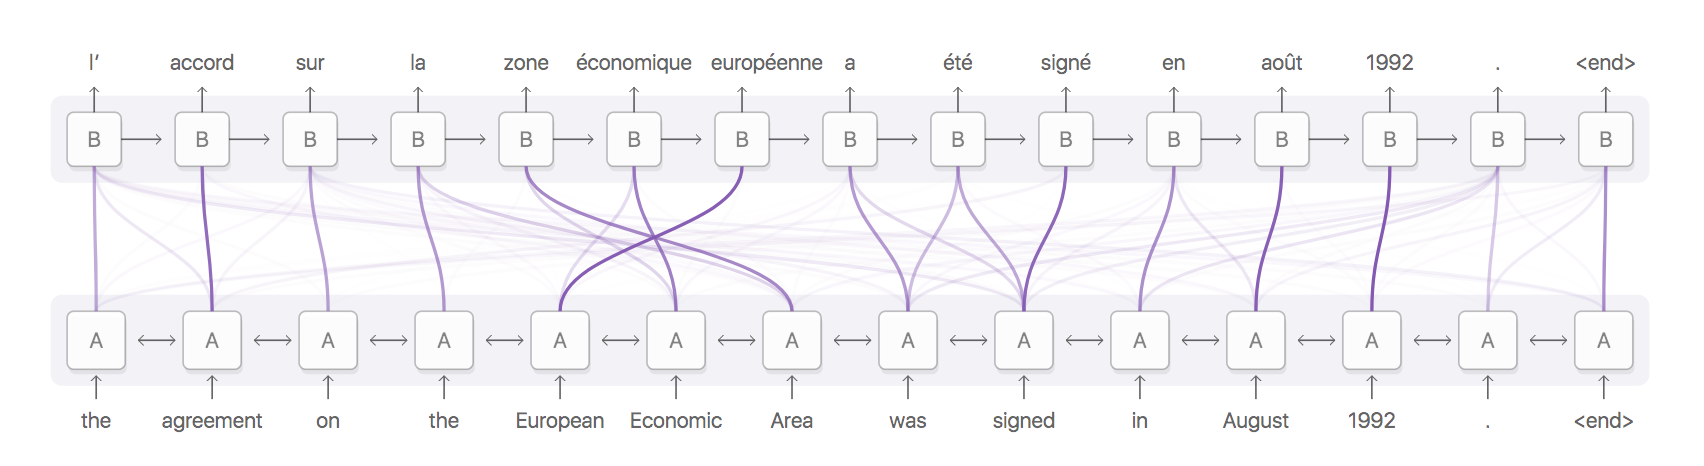
\includegraphics[width=1\textwidth]{wordattn}
  \caption[Attentional word diagram for English to French Translation]{When translating, certain words in the input will have a disproportionate effect on words in the output. From~\cite{Olah2015} with permission.}
  \label{fig:wordattn}
\end{figure}

To address this, an attentional framework was developed in 2014~\cite{Bahdanau2014}. The original attentional model can be thought of as a simple neural net between the encoder and decoder that attempts to determine the strength of the influence that words in the starting sequence will have on a particular output~\cite{Bahdanau2014}. This was further developed upon in 2015 by implementing different scoring functions~\cite{Luong2015}, the specifics of which are outside the scope of this literature review. Attentional decoders have proven their effectiveness and are used in all sophisticated seq2seq models today, including headline generation.

\subsubsection{Seq2Seq Conclusion}
RNN encoders fed into attentional RNN decoders represent the architectural framework of the state-of-the-art. Note that the encoder and decoder RNNs can a multiple layers deep by feeding the output of an encoder into another encoder and vise versa. For example, the Neural Machine Language architecture behind Google's Translate service uses 8 encoders and 8 decoder~\cite{Wu2016}. These allow for far more complex characteristic representations at the cost of far greater training time and computation requirements.

\subsection{Teacher Forcing}\label{tf}
The last piece to understand is the concept of teacher forcing (TF)~\cite{Williams1989}. In Figure~\ref{fig:seq2seq}, there is a grey arrow on the right side of the diagram pointing from the \textit{output} of the decoder back to the \textit{input} of the decoder. This is how a trained RNN will generate a sequence. However, when a model's weights have not yet been trained, this is highly ineffective as the output at any given timestep will almost certainly be incorrect. The decoder will then attempt to modify its weights for subsequent time steps based upon an incorrect prior state, which theoretically should result in much longer training time. To combat this, teacher forcing was developed~\cite{Williams1989} which instead feeds the correct, labeled output back into the decoder regardless of how it predicted the previous timestep.

It was noted, however, that models which were constantly fed the correct prior state were not functioning as well at inference time. It was theorized that this was because the model had developed a dependency on receiving the correct prior state~\cite{Bengio2015}, but it wasn't until 2015 that this was addressed with a technique called scheduled sampling~\cite{Bengio2015}. In the models that have been created for headline generation, however, TF has been a binary decision---either always feed the decoder the input or don't at all. This is because the deep learning frameworks used in state-of-the-art models, namely tensorflow and torch, all require pre-defining the neural network's computational graph before runtime, which does not allow the flexibility required for dynamic teacher forcing~\cite{Howard2017}.

However, a relatively new deep learning library called PyTorch builds the computational graph at run-time~\cite{Chintala2017} and is consequently far more customizable~\cite{Howard2017}. As a result, dynamic teacher forcing can now be implemented and it is the aim of this dissertation to explore the effect of these various TF techniques on model performance.